%%%%%%%%%%%%%%%%%%%%%%%%%%%%%%%%%%%%%%%%%%%%%%%%%%%%
%												   %
%                                   			   %
%   Antoine Faravelon, Lucas Felix,                %
%   Miratul Khusna Mufida, Hugo Guiroux,           %
%   Simon Moura                                    %
%												   %
%%%%%%%%%%%%%%%%%%%%%%%%%%%%%%%%%%%%%%%%%%%%%%%%%%%%

\documentclass[a4paper,10pt]{article}
\usepackage{amsthm}
\usepackage{amsmath}
\usepackage{amsfonts}
\usepackage{mathtools}
\usepackage{wrapfig}
\usepackage{graphicx}
\usepackage{titling}
\usepackage{float}
\usepackage{caption}
\usepackage{subcaption}
\usepackage{listings}
\usepackage{fullpage}
\lstset{%
    basicstyle=\scriptsize\sffamily,%
    commentstyle=\footnotesize\ttfamily,%
    frameround=trBL,
    frame=single,
    breaklines=true,
    showstringspaces=false,
    numbers=left,
    numberstyle=\tiny,
    numbersep=10pt,
    keywordstyle=\bf
}
\newcommand{\subtitle}[1]{%
    \posttitle{%
        \par\end{center}
    \begin{center}\large#1\end{center}
\vskip0.5em}%
}

\newcommand{\CCscript}[2]{
    \begin{itemize}
        \item[]\lstinputlisting[caption=#2,label=#1,language=CC]{src/#1.cc}
    \end{itemize}
}
\lstdefinelanguage{codeoutput} { %this is the name that you are going to use when you want to use the formatting
    basicstyle=\ttfamily\scriptsize, %font family & size
}
\newcommand{\Oscript}[2]{
    \begin{itemize}
        \item[]\lstinputlisting[caption=#2,label=#1,language=codeoutput]{src/#1}
    \end{itemize}
}
\newcommand{\Cscript}[2]{
    \begin{itemize}
        \item[]\lstinputlisting[caption=#2,label=#1,language=CC]{src/#1.c}
    \end{itemize}
}

\setlength{\abovecaptionskip}{1pt plus 1pt minus 1pt} % Chosen fairly arbitrarily

\title{Nachos}
\subtitle{Project [MOSIG - M1]}
\author{Antoine Faravelon, Lucas Felix, Miratul Khusna Mufida, Hugo Guiroux, Simon Moura}
\date{\today}

\begin{document}
\maketitle

\section{network implementation}
	We chose to implement a socket user interface in our Nachos kernel. These sockets work in connected mode with robust transmissions.
As in Unix TCP sockets, a server create a listening socket and accept new connections on it. This allow to join a server on one port (defined by convention as 80 for HTTP server) with many clients, and each of them will then have a personal socket with the server.
On its side, the server can communicate with each client separately on different sockets.
Our kernel provides 16 ports which can handle 16 sockets each, so the kernel can handle 256 connections at a time.

\subsection{Low level transmission}
	The lower layer of our network implementation is the transmission of one mail. This part have to be robust and then we can construct an higher level protocol on it.
For every single mail, the emitter send the mail, wait a confirmation and retry if no. The number of tries is limited and the send function will return an error if this limit is reached.

The receiver can receive many times the same mail before the emitter receive a confirmation. To prevent the duplication of a mail, we include an id in each of them. The receiver will take the first iteration of a mail and just confirm the other ones.
The id we use is an int which is always incremented, so the network will stop to work after $2^{32}$ mails sent. This limit is hard to reach, so we did not deal with it, but it is possible to make the id go back to 0 when it happens without blocking the network.
A confirmation mail contains the id of the mail it confirm, so a confirmation mail cannot be used later by the emitter to confirm an other sending.

\subsection{Protocol}
	The protocol we constructed on the robust transmission level is connected (like TCP). The connection establishing is not symmetric (there is a server and a client) and use a three-way handshake.
We use the mailboxes of the initial Nachos code as ports, but now each mailbox contains an array of socket because many sockets can be connected within a same port (for instance the port 80 of HTTP servers).
The number of connections a port can handle is limited to 16, because an array was simpler to implement and 16 is sufficient (but it can be replaced easily by a list).

The postal worker dispatch the mails he receive. He know in which mailbox thanks to the mail header and then find the good socket by comparing the origin of the mail to the ones contained into sockets.

--------------------------IMAGE--------------------------
%\begin{figure}[H]
%	\centering
%		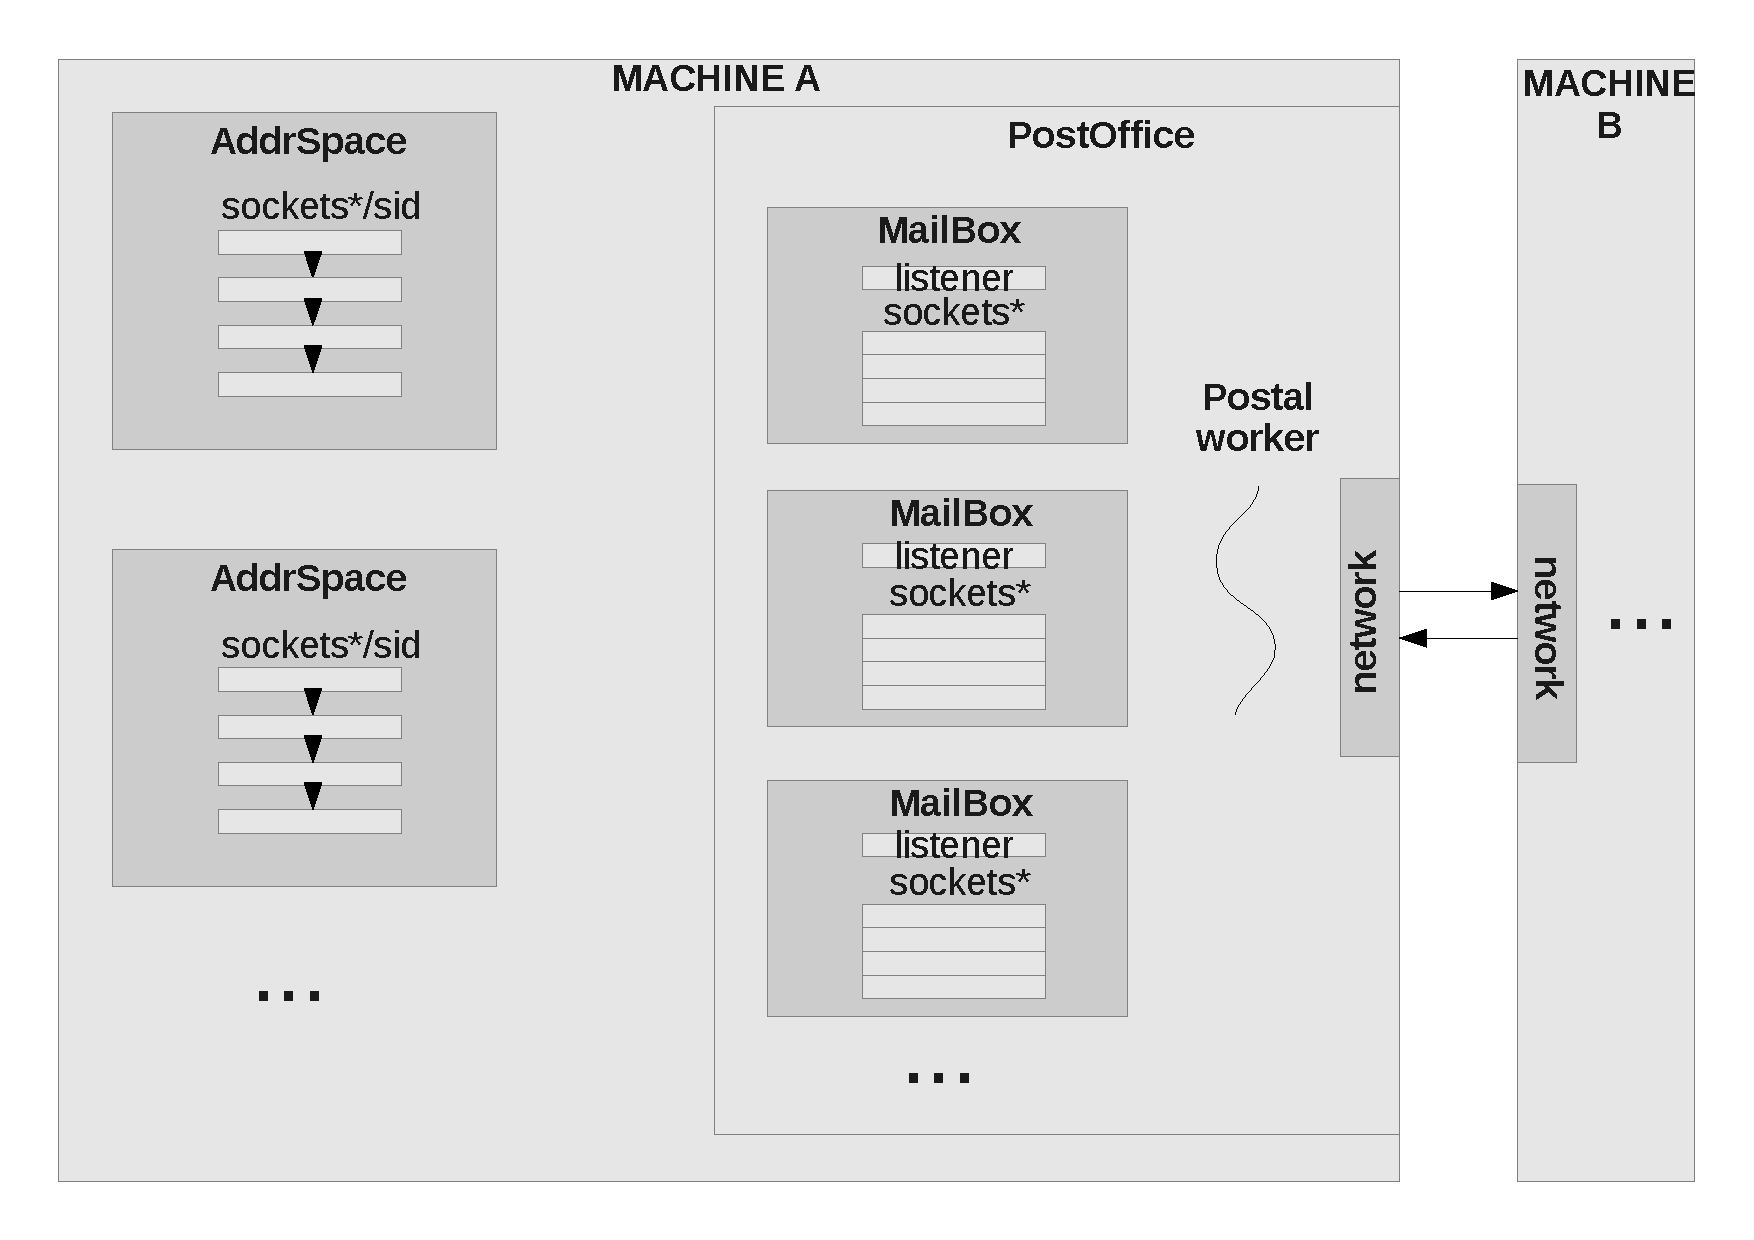
\includegraphics[scale=0.55]{networkschema}
%\end{figure}

\end{document}
